% !TeX root = ..\main.tex
% !TeX program = xelatex

% Chapter 1
\chapter{绪论}

本章主要介绍研究背景与意义、中文古诗生成相关的研究现状,阐述本论文的研究思路与主要贡献,并介绍论文的组织架构。

\section{研究背景和意义}

文本生成任务(Text Generation)是自然语言处理(Natural Language Processing, NLP)的一个重要研究方向,需要在给定输入或上下文的条件下,输出符合要求的文本,涵盖机器翻译、文本摘要、对话生成、作品创作等多个应用方向。而在文本生成领域中,中国古代诗歌的生成更是一个困难的任务。

古诗是中华传统文化的瑰宝,作为最早形成的中国古代文学作品体裁之一,其措辞简洁、内涵丰富且韵律整齐。中国古诗的典故意象运用极具文化特色、用词凝练优雅,这些独特的艺术特色都为古诗的机器创作带来巨大的挑战。如何让机器模型深入理解并创作出具有文化内涵和艺术价值的古诗,继而为中华传统文化的再创造赋能,是一个富有挑战的有趣问题。

早期的古诗生成主要依赖于其他子领域的研究思路。例如,\cite{oliveira2012poetryme}利用现有古诗作为模板,根据既定规则替换字词来生成新的古诗,这样生成的古诗虽在形式上合格,但表达力欠佳;\cite{yanPoetAutomaticChinese2013}将其看作是一个摘要生成任务,只是输入是作者的表达意图,且需要考虑中文古诗独特的韵律形式约束;\cite{heGeneratingChineseClassical2012}则将其看作一个机器翻译任务,将古诗的上下句子分别看作是翻译的源语言和目标语言,利用统计机器翻译(Statistical Machine Translation, SMT)的方法来生成古诗。

随着深度学习技术的发展,近年的中文古诗生成大多将古诗生成视作是“从序列到序列”的预测任务(Sequence-to-Sequence),并由此出发训练循环神经网络(Recurrent Neuro Networks, RNNs),如编码器-解码器(Encoder-Decoder)模型\cite{yiGeneratingChineseClassical2017},并以此为基础设置额外机制来增强语义表现\cite{zhangChinesePoetryGeneration2014}或韵律格式约束\cite{liRigidFormatsControlled2020,huPoetryDiffusionJointSemantic2024}。然而,这些方法对古诗内涵的掌握往往停留在上下文语义或是韵律对仗,无法进一步触达诸如典故、意象和全诗连贯性等更复杂的方面。所幸,大模型(Large Model, LM)展现出强大的语义理解与创作能力,而在中文领域也出现了诸如ERNIE\cite{zhangERNIEEnhancedLanguage2019}、DeepSeek-R1\cite{deepseek-aiDeepSeekR1IncentivizingReasoning2025}这样的大语言模型(Large Language Model, LLM)和DeepSeek-VL\cite{luDeepSeekVLRealWorldVisionLanguage2024}等跨模态大模型,为这一领域注入全新的活力。\cite{yuCharPoetChineseClassical2024}

除了文本输入外,中国古诗往往蕴含着丰富的场景意象,其对应的视觉信息难以通过用户输入来精确描述。目前也有方案直接使用图像作为输入,如在循环神经网络外增加卷积神经网络(Convolutional Neuro Networks,CNNs)以处理图像信息,捕捉图像关键主体并把握整体氛围,最终生成古诗。\cite{liuImages2PoemGeneratingChinese2018,xuHowImagesInspire2018}但相应地,这些方案放弃了文本输入能够具体描述要求的优势,输入图像所含信息的繁杂也导致生成古诗主题、内涵乃至风格的波动。现有的方案大都局限于或文本或图像的单一模态输入,要么局限于上下文语义或韵律的形式规律而无法触达更高的艺术层次,要么受制于图像信息的多变而无法实现更精细的输出控制。这种单一模态的输入限制了用户描述需求的可能,也使生成的古诗缺乏层次,这暗示着文本“跨模态”输入的研究方向,也是本选题希望探讨的内容。

另一个重要的问题是生成结果的“可解释性”(Interpretability),指系统以人类可理解的术语解释或呈现模型行为的能力。\cite{doshi-velezRigorousScienceInterpretable2017}深度学习技术在带来更高表现的同时,其“黑盒”的特性也使得可解释性问题愈发突出。在古诗生成任务中,可解释性可体现为三个方面:

\begin{enumerate}[label=(\arabic*), itemindent=2em]   % lefrmargin=2em表示左边距,itemindent=2em表示序号缩进
    \item 过程可解释性,即系统是如何从输入的文本和图像中提取信息,并进一步并生成古诗的,其中包含哪些中间步骤;
    \item 结果可解释性,即系统为何生成这样的古诗结果,其中遵守怎样的韵律形式、又运用了哪些典故意象;
    \item 反馈可解释性,即系统如何分析生成古诗的质量,如何让用户理解古诗“好坏在哪里”。
\end{enumerate}

现有的古诗生成系统大多缺乏对生成过程的可解释性,用户难以理解系统是如何从输入信息中提取出关键信息并生成古诗的;而在结果可解释性方面,现有的系统也往往只提供了生成古诗的文本,而没有进一步解释其韵律、意象等方面的内涵;在反馈可解释性方面,现有的系统也缺乏对古诗质量评价维度的详细说明,用户需要具备较高的文学素养以理解和甄别对古诗质量的评价。因此,提升古诗生成系统的可解释性,将有助于增强用户对系统的信任感和使用体验,使得用户能够更好地理解和利用系统输出的古诗和相应的质量判断。

本文旨在探讨文图跨模态的中文古诗生成,开发了一个基于大模型的古诗创作系统。在给定用户两种模态输入的条件下,其能够通过图像的分析描述来充分提取图像信息,结合用户输入的文本信息,生成符合古诗韵律和意象的古诗。此外,系统还将提供对古诗的分析文本、量化评分以及改进意见,涵盖韵律对仗、典故意象、主题思想、语言用词等多个赏析方面,并支持多轮迭代优化。

\section{研究现状}

\subsection{中文古诗生成}
近年来,中文古诗生成领域引起了广泛的研究兴趣。2016年,\cite{wangChinesePoetryGeneration2016}使用修改的注意力结构的编码器-解码器模型来解决古诗生成过程中主题漂移的问题,但限制关键词的数量和顺序,降低了系统的灵活性。这一问题在2018年由\cite{xuHowImagesInspire2018}通过记忆网络(增加记忆组块的RNNs)基于图像生成古诗解决。2020年,\cite{WangJiYuSeq2SeqMoXingDeZiDingYiGuShiShengCheng2020}将注意力机制引入了Seq2Seq模型,实现了基于关键字的自定义古诗生成。

古诗的生成可能会出现多方面的质量波动,包括主题、语言风格、字数格式、韵律对仗等等,需要在研究中纳入考量。2020年,\cite{liRigidFormatsControlled2020}设计了一个基于Transformer的自回归模型,改进注意力机制并进一步收紧了包括中文古诗、歌词、英文十四行诗等特殊文体生成的格式要求。2021年,\cite{wuGenerateClassicalChinese2021}从图像中提取物体关键词、情感和风格,以生成古诗。\cite{shaoSentimentStyleControllable2021}将数十万首古诗按照风格、情感、格式与主要关键词分类,并利用掩蔽自注意力机制来建立标签到诗句的关联,以此来生成情感与风格均可控的古诗。2022年,\cite{LiFengGeHeQingGanKongZhiDeZhongGuoGuShiShengCheng2022}将GAN中的判别器与生成器结构加入到CVAE中,实现对风格和情感的控制。2023年,\cite{renGeneratingChinesePoetry2023}构建了一个古诗图像数据集,精确标注了其中的诗歌元素,并利用GRU网络来增强生成古诗的上下文关联。2024年,\cite{huPoetryDiffusionJointSemantic2024}首次使用扩散模型来生成古诗,以实现对语义与韵律的同时控制。

后来逐渐出现使用LLM生成古诗的方案。2024年,\cite{CengShengChengShiYuYanMoXingZaiGuShiShengChengZhongDeYouHua2024}通过强化学习算法PPO对GLM模型进行训练,提升其在古诗生成方面的表现。\cite{yuCharPoetChineseClassical2024}修正了LLM以token计数会导致输出格式错误的问题,改以字符计数,达到了极高的格式精度。\cite{liuMultiModalChinesePoetry2018}则提出了一种图片输入的三段式绝句生成方法,将短语特征纳入考量,并构建了一个图像主题数据集。其将输入的图片映射到一个主题词,再随机选择与该主题词相关的短语,再通过一正一反两种方向的LLM来依次生成古诗的首行、标题和其他主体内容。

值得注意的是,鲜有研究关注文图跨模态的古诗生成。据调研,目前只有\cite{liuDeepPoetryChinese2020}一项研究同时包含文本和图像两种模态的输入,其通过Clarifai来将图像映射到两个具体的主题词,根据这两个主题词在已有短语库中进行检索拓展,再进一步将得到的短语通过一个自注意网络来生成古诗。这一系统允许用户来限制古诗的诗句前缀词,因此可广义地认为实现了图文的跨模态输入。

\subsection{古诗质量评价}
如何评价生成古诗的质量是一个难题,考虑到古诗体裁的艺术性,其质量评价往往依赖于人工评估。除此之外,也可使用以往文本生成的自动度量方法,如源自机器翻译领域基于$n$-gram\footnote{表示文本中连续的$n$个词或字符。如“我爱你”中基于字符的$2$-gram集合为[“我爱”、“爱你”]}的翻译文本评估方法
BLEU\cite{papineniBLEUMethodAutomatic2002}和ROUGE\cite{linROUGEPackageAutomatic2004}。其中,BLEU指标计算生成文本中有多少$n$-gram出现在参考文本中,即使用精确率(Precision)来评估生成文本有多接近参考文本;相反,ROUGE指标计算参考文本中有多少$n$-gram能够被生成文本包含,即使用召回率(Recall)来评估生成文本能否完整地覆盖参考文本。可见,BLEU和ROUGE指标均依赖于与高质量参考文本的对比。此外,Distinct\cite{liDiversityPromotingObjectiveFunction2016}基于$n$-gram的多样性来评估生成古诗的多样性,即诗句里有多少不同的$n$-gram。而为了评估上下文语义的一致性,Similarity\cite{wietingUniversalParaphrasticSentence2016a}使用词向量来计算句子之间的相似度。这些方法都能脱离参考文本独立地评价文本质量。

除了自动度量方法外,也有一些研究实现了对古诗的质量优化。2020年,\cite{dengIterativePolishingFramework2020}提出一个质量感知的掩蔽语言模型,实现一个可迭代的古诗优化框架,可用于判断古诗是否需要优化,并在润色时定位不恰当部分。2023年,\cite{maYuShengHumaninLoop2023}提出一种人机协作的古诗创作系统,能够在不同的约束条件下对古诗进行润色。2024年,\cite{chenPolishingModelMachineGenerated2024}又提出了一个可迭代的古诗优化框架,基于BiLSTM和CRF构建用于检测低质量用词的检测网络、基于BERT模型构建用于修正用词的校正网络。这些研究均实现了“评价+优化”的流程功能,且效果良好。美中不足的是未提供对“评价”本身的解释,即“被选中的词为何是低质量的,而优化又依据着什么”的问题。

\subsection{大模型技术}
近年来,大模型技术取得了显著的进步,其中以大语言模型最为典型,例如OpenAI开发的生成预训练转换器(GPT)系列模型、百度开发的知识整合增强表示(ERNIE)系列模型\cite{zhangERNIEEnhancedLanguage2019}。DeepSeek开发了首个通过强化学习训练的大语言模型 DeepSeek-R1\cite{deepseek-aiDeepSeekR1IncentivizingReasoning2025},其采用混合专家模型(Mixture-of-Experts, MoE)架构,实现在相同计算成本下大幅提升模型的参数规模与推理能力。

而与LLM擅长自然语言类似,还有许多跨模态大模型适用于不同模态间数据的信息表征处理,如文本和图像。由OpenAI开发的CLIP模型\cite{radfordLearningTransferableVisual2021}包含一个文本解码器和一个图像解码器,在大量图像及其对应的文本描述的数据集上进行预训练,因而能够把握视觉表征与文本之间的关联。MiniGPT-4\cite{zhuMiniGPT4EnhancingVisionLanguage2023}是GPT-4模型的缩小版,它将一个与BLIP-2架构相同的视觉编码器与语言模型Vicuna通过一个单一的投影层链接起来,在图像描述生成方面展现出卓越的能力。
DeepSeek开发的DeepSeek-VL\cite{luDeepSeekVLRealWorldVisionLanguage2024}的训练数据来自广泛的现实场景,其采用了一个混合视觉编码器,可在固定的token预算内有效处理高分辨率图像,同时保持相对较低的计算开销,这一设计选择确保了模型在各种视觉任务中捕捉关键语义和详细信息的能力。有趣的是,DeepSeek-VL在一开始便整合了LLM的能力训练,促进视觉和语言两种模态能力的平衡整合,使其在能够捕捉视觉语义信息的同时,仍然具有强大的语言能力。在此基础上,DeepSeek-VL2\cite{wuDeepSeekVL2MixtureofExpertsVisionLanguage2024}进一步改进了视觉与文本的能力整合。视觉上融入动态分块的编码策略以处理不同比例尺寸的图像,文本上则引入了MoE架构,可动态选择专家模型完成不同的任务。

\subsection{提示工程}
提示工程逐渐作为一种通过自然语言来调整和控制LLM行为的技术。目前人们已提出多种提示词的设计原则与策略。Few-shot框架\cite{brownLanguageModelsAre2020}为模型提供少量示例样本,以有效地指示模型完成指定任务。思维链(CoT)框架\cite{weiChainofThoughtPromptingElicits2022}指导模型将任务分解为若干子任务来逐步完成,使模型能在无其他修改的情况下完成复杂的因果推理任务。自洽性(Self-Consistency)\cite{wangSelfConsistencyImprovesChain2023a}旨在小样本CoT中对多种推理路径进行采样,并在尝试生成之后选择最一致的答案,其有助于提高CoT提示在涉及算术推理和常识推理的任务中的性能。此外,开发者们也提出了十分多样的提示词框架,例如CRISPE、ICIO、BROKE,均经过了开源社区的检验,令人目不暇接。

\section{研究思路和主要贡献}

本选题旨在利用大模型的通用能力,设计并实现一个文图跨模态的中文古诗创作系统:1)分析输入的图像,生成易使用的描述文本,兼顾关键物体与整体氛围;2)设计评判标准,设计提示词分别用于古诗生成和分析,调用模型生成古诗、分析结果与改进意见;3)结合已有的质量评价维度和其他系统,设计实验验证古诗分析分数、跨模态生成对古诗质量影响的效度,并探索系统改进方向。

\begin{figure}[ht]
  \centering
  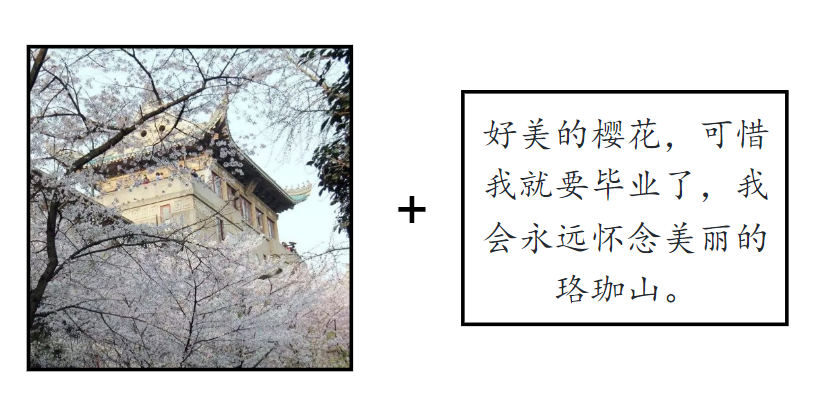
\includegraphics[width=0.65\textwidth]
  {figures/示例输入.png}\\
  \caption{示例输入}
  \label{fig:example_input} % 添加标签
\end{figure}

为处理输入的图像模态,需要使用跨模态能力优良的视觉与文本编码模型。在先前的工作中,使用CLIP模型来识别图像中的物体,使用MiniGPT4模型来生成初步的图像描述,之后再由ERNIE-4.0结合二者生成最终的中文描述文本。诚然,CLIP与MiniGPT4模型均具备极强的视觉与文本的映射能力,但二者均属英文模型,缺乏中文文化语境的训练,因而难以捕捉图像中潜在的文化意味与情感,这部分缺乏的信息难以在ERNIE-4.0模型的总结中恢复,从而影响古诗生成的质量。为此,本文采用在中文语境下训练的模型来处理图像模态,经初步对比,DeepSeek-VL模型生成的图像描述文本更具诗意美感,且在古诗生成的质量上也更具优势,因而本文将使用DeepSeek-VL模型来处理图像模态。(输出如图~\ref{fig:image_description})

\begin{figure}[ht]
  \begin{tcolorbox}[
      colback=white, % 背景透明
      colframe=black, 
      boxrule=1pt,        % 设置边框宽度
      arc=0mm,             % 取消圆角
  ]
      \kaishu 这张图片展示了一座传统中式建筑,其屋顶装饰着精美的绿色琉璃瓦,显得庄重典雅。建筑主体为浅黄色,四周有栏杆围绕,似乎有游客站在阳台上欣赏风景。前景是繁茂的樱花树,粉白色的花朵覆盖了大部分画面,营造出浪漫而宁静的氛围。天空清澈,与花朵的柔和色彩形成鲜明对比,增添了画面的层次感。整幅画面让人感受到春天生机勃勃的气息,同时也透露出一种悠闲和诗意的情感。
  \end{tcolorbox}
  \caption{图像描述(示例)}
  \label{fig:image_description} % 添加标签
\end{figure}


古诗具有独特的韵律格式要求,如平仄、押韵、对仗等要求,且注重典故与意境协调。在先前的工作中,使用ERNIE-4.0模型来生成古诗,虽能基本遵守韵律格式要求,但无法兼顾典故运用和意境圆满。为此,本文使用基于强化学习训练的DeepSeek-R1模型(生成古诗如图~\ref{fig:example_poem}),其链式的推理过程包含对多种候选推理路径的动态评估和筛选,能够在反复验证中确保生成古诗的韵律要求,并且也展现了对典故意象的更强运用能力。这一能力也有助于提高系统的可解释性,为用户输出更合理清晰的解释性文本,包括白话文翻译、古诗赏析和典故注释。(如图~\ref{fig:example_translation}、~\ref{fig:example_appreciation}和图~\ref{fig:example_annotation})

\begin{figure}[ht]
  \centering
  \begin{tcolorbox}[
      colback=white,
      colframe=black,
      boxrule=1pt,
      arc=0mm,
      width=0.6\linewidth,  % 控制宽度
      ]
      \kaishu
      \centering
      珞珈山下琼英绽,朱阁檐前翠影摇。\par
      万点飞花迷画槛,千重香雪覆虹桥。\par
      琉璃映日浮金阙,玉砌连云接碧霄。\par
      曲径曾携书卷过,长亭忍看落英飘。\par
      东君不解离人恨,更遣残红逐晚潮。\par
      粉泪暗随春水逝,青衿空对暮山遥。\par
      他年若问芳菲事,犹记晴川鹤影娇。\par
  \end{tcolorbox}
  \caption{生成古诗(示例)}
  \label{fig:example_poem}
\end{figure}


\begin{figure}[ht]
  \centering
  \begin{tcolorbox}[
      colback=white,
      colframe=black,
      boxrule=1pt,
      arc=0mm,
      width=0.8\linewidth,  % 控制宽度
      ]
      \kaishu
      \centering
      珞珈山下樱花绽如琼瑶,朱红楼阁前翠影正轻摇。\par
      万点飞花迷蒙了雕栏画柱,千层香雪压弯了求学虹桥。\par
      琉璃瓦映日似浮动金殿,白石阶入云直通向碧霄。\par
      曾捧书卷走过这林荫曲径,长亭外怎忍看落英飘摇。\par
      春神不懂人间别离苦楚,偏让残红追着晚潮远漂。\par
      粉泪默默随春水流逝去,青衫空对暮色里的山遥。\par
      若问当年花开烂漫旧事,定记得晴川上鹤影正娇。\par
  \end{tcolorbox}
  \caption{古诗白话文翻译(示例)}
  \label{fig:example_translation} % 添加标签
\end{figure}

\begin{figure}[ht]
  \begin{tcolorbox}[
      colback=white, % 背景透明
      colframe=black, 
      boxrule=1pt,        % 设置边框宽度
      arc=0mm,             % 取消圆角
  ]
      \kaishu 这首七言排律以武大樱花为情感载体,通过工丽的对仗与典雅的意象,构建出毕业离别的双重意境。首联以"琼英""翠影"点题,既暗合《诗经》"尚之以琼英乎而"的典故,又呼应图片中琉璃瓦与樱花的色彩映照。颔联"万点飞花"与"千重香雪"形成空间纵深感,化用岑参"千树万树梨花开"的意境而翻出新意。颈联转写建筑,“琉璃映日"直取图片意象,“玉砌连云"暗用李煜"雕栏玉砌"之典,将现代学府与传统意象完美融合。尾联"晴川鹤影"既化用崔颢"晴川历历汉阳树”,又暗喻学子如鹤高飞,留下余韵悠长的想象空间。全诗严守平水韵,中二联"迷画槛"对"覆虹桥”,“浮金阙"对"接碧霄”,工稳中见灵动,以物象变迁写时光流逝,最终在"鹤影"的意象中完成对母校记忆的诗意定格。
  \end{tcolorbox}
  \caption{古诗赏析(示例)}
  \label{fig:example_appreciation} % 添加标签
\end{figure}

\begin{figure}[ht]
  \begin{tcolorbox}[
      colback=white, % 背景透明
      colframe=black, 
      boxrule=1pt,        % 设置边框宽度
      arc=0mm,             % 取消圆角
  ]\kaishu
      1. 琼英:取自《诗经·齐风》“尚之以琼英乎而”,既指樱花如玉,又喻学子才俊\par
      2. 朱阁:对应图片中浅黄色建筑,化用苏轼"转朱阁"意象,暗喻学术殿堂\par
      3. 虹桥:既实指校园拱桥,又暗用《东京梦华录》虹桥典故,喻求学之路\par
      4. 琉璃:特指图片中绿色琉璃瓦,呼应白居易"琉璃波面月"的华美意象\par
      5. 玉砌:化用李煜"雕栏玉砌应犹在",将现代建筑古典诗化\par
      6. 东君:司春之神,此处双关东风与毕业季的时令特征\par
      7. 青衿:源自《诗经》“青青子衿”,既指学子装束,又喻求知初心\par
      8. 晴川鹤影:化用崔颢"晴川历历汉阳树","鹤"取《诗经》"鹤鸣于九皋"意象,喻志向高远\par
      9. 香雪:借李商隐"匝路亭亭艳"咏樱花之意,特指白色樱花如雪\par
      10. 画槛:对应图片中栏杆意象,暗用"画栋朝飞南浦云"的滕王阁典故\par
  \end{tcolorbox}
  \caption{古诗注释(示例)}
  \label{fig:example_annotation} % 添加标签
\end{figure}





为有效地评估生成古诗的质量,本文设计了一个包含多维度的评分体系,以进行量化评分并促进优化方案的梳理。在之前的工作中,基于六个方面\footnote{包含“结构与形式”、“语言与风格”、“意象与主题”、“协调与一致”、“历史语境”、“创新性”}设计提示词,其中对每个方面进行简要描述,并使用ERNIE-4.0模型打分。在测试时发现,这样的评分体系无法提供标准化的分数,输出的分数整体偏高,区分度差。因此,本文重新设计了一个包含五个方面\footnote{包含“格律规范”、“意象意境”、“主题思想”、“语言锤炼”、“创新性”}的评分体系,不同于之前对各方面的简要描述,其给出了各分数段的情况描述,并附上了具体例子(如表~\ref{tab:poem_scoring}),有效地提升了评分结果的区分度和合理性,也为后续的优化方案提供了更清晰的方向。而作为补充,本文也将利用BLEU、ROUGE、Distinct、Similarity等指标辅助古诗质量的评估。



本研究的主要贡献在于探索了大模型在中文古诗生成中的应用潜力,结合文图两种模态来强化生成古诗与用户需求的契合度,期间提供用户友好的解释性文本,使得用户更易理解和信任机器生成的创作过程及其背后的文化内涵;同时,设计评分体系来输出量化结果,在促进古诗的多轮优化的同时进一步提高系统可解释性。本研究有助于拓展和弘扬中华传统文化的表达形式,推动诗词创作与人工智能技术的深度融合,具有重要的理论意义和实践价值。

\section{论文组织结构}

    第一章是概论部分。
    
    第二章介绍古诗生成任务的现有技术,对古诗的基本要求、自动度量方法、DeepSeek大模型等进行概述。

    第三章介绍本系统的设计与实现,对整体架构、各个模块的功能和实现方法进行概述。

    第四章介绍开展实验的设计与结果分析,基于已有古诗数据集,结合自动度量方法来评估系统,并展开分析论述。

    第五章是结语,对本文的工作内容进行总结,并探讨局限性与改进空间。